\section{Marco Teórico}

\subsection{Meteorología}

La meteorología es la ciencia encargada de estudiar

\subsection{Datos meteorológicos}

La guía para los instrumentos meteorológicos y métodos de observación (conocida como la guía \textit{CIMO}), publicada por la Organización Meteorológica Mundial (\textit{WMO} en adelante) establece una serie de criterios y estándares \cite{CIMO_2008} que deben ser utilizados para la definición, recolección y uso de los datos meteorológicos.

\subsubsection{Temperatura}
La WMO \cite{CIMO_2008} define como temperatura como una cantidad física que caracteriza el movimiento aleatorio de moléculas en un cuerpo físico. Para fines meteorológicos, se toma la temperatura media como punto de medición, y comúnmente se mide la temperatura del aire a diversas altitudes. Sin embargo, también son utilizadas otras temperaturas, como la de el suelo, la tierra y la temperatura de el agua marina. En el caso de la temperatura del aire, esta se define como la temperatura de un termómetro en un expuesto al aire pero cubierto de la luz directa del sol.

\subsubsection{Presión atmosférica}

La presión atmosférica es definida por la WMO \cite{CIMO_2008} como la cantidad de presión ejercida por la atmósfera en un punto, en medida de fuerza por unidad de área. Además de la presión, la WMO también recomienda el calcular la tendencia de la presión. Esta es definida como la cantidad de cambio de presión en un lapso de 3 horas.

\subsubsection{Velocidad y dirección del viento}

La velocidad del viento es un vector tridimensional de cantidad con variaciones pequeñas aleatorias, y caracterizado por fluctuaciones rápidas llamadas ráfagas. Generalmente se utiliza la representación polar del promedio de velocidad horizontal del viento, y su dirección como dato meteorológico \cite{CIMO_2008}.

\subsubsection{Humedad específica y relativa}

La humedad específica es el radio entre la masa de vapor de agua y la masa de aire húmedo. en camboi, la humedad relativa es el radio entre el porcentaje de la presión observada del vapor y la saturación de la presión del vapor con respecto al agua a la misma temperatura y presión.

\subsection{Estacion meteorológica}

\subsection{Redes Meteorológicas Urbanas}

Las redes meteorológicas urbanas, son una metodología de recolección de datos especialmente útil para ambientes de población urbanos con una densidad alta, que requiere de una cantidad considerable de sensores distribuidos . Muller \textit{et al} \cite{doi:10.1002/joc.3678} describen las redes meteorológicas urbanas como un

% \begin{figure}[ht!]
%    \centering
%    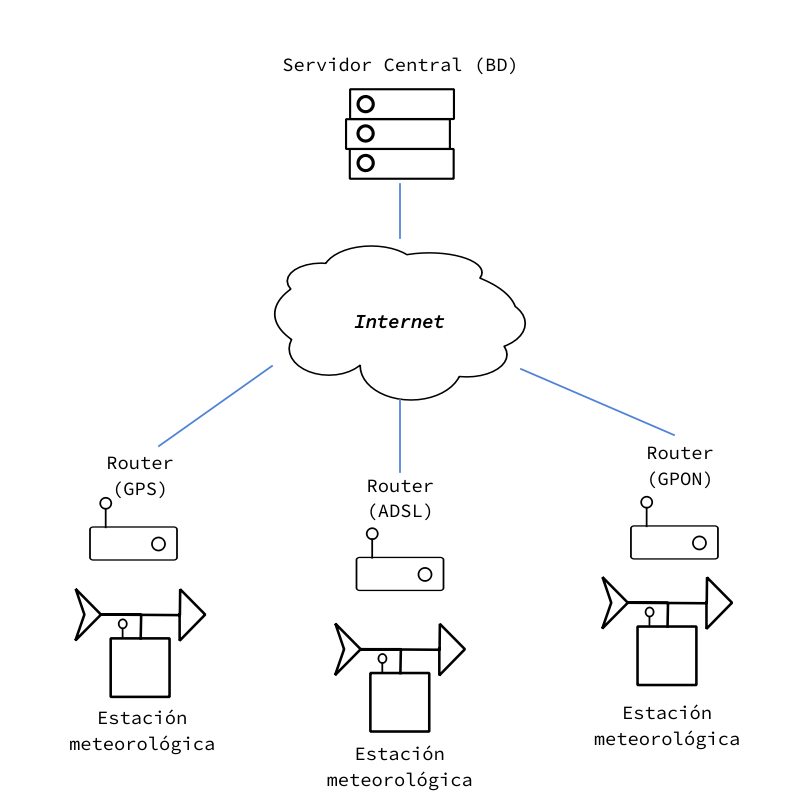
\includegraphics [ width = 0.8\textwidth ] {images/stations_arrangement.png}
%    % 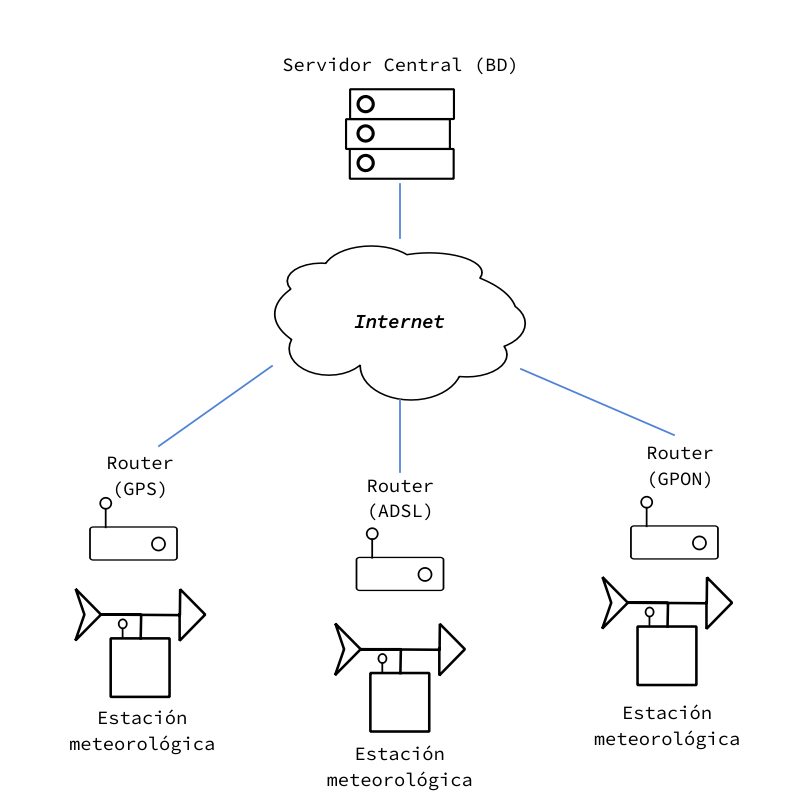
\includegraphics [ height = 160px ] {images/stations_arrangement.png}
%    \caption{Organización de las estaciones meteorológicas en el laboratorio CECATEV de la UACJ}
%    \label {fig:stations}
% \end{figure}

Sensores

Tiempo de actualizacion de datos, por variables fisicas.
\cite{davis:6152C_6162C_SS}.

\subsection{Transformada de ondícula}



\subsection{Métodos de compresión}

La compresión de datos se realiza por medio de diversas

   Ruido
      Reducción de ruido
      Normalización de temperatura por medio de Filtros
   Fourier

